\chapter{Laboratorio 5}
Il primo circuito realizzato in questa esperienza di laboratorio permette di effettuare lo switch debouncing attraverso l'integrato LM555. Nella figura \ref{fig:circuito_1} è riportato lo schema del circuito.
\begin{figure}[h!]
	\centering
	\begin{minipage}{.45\textwidth}
		\scalebox{.47}{
			\begin{circuitikz}
				%Main dip package
				\draw (0,0) node[dipchip,num pins=8, hide numbers, external pins width=0.1, scale=3, external pad fraction=6](C){LM555};
				%Pin names
				\node [right] at (C.bpin 1) {GND};
				\node [right] at (C.bpin 2) {Trigger};
				\node [right] at (C.bpin 3) {Output};
				\node [right] at (C.bpin 4) {Reset};
				\node [left] at (C.bpin 5) {Control Voltage};
				\node [left] at (C.bpin 6) {Threshold};
				\node [left] at (C.bpin 7) {Discharge};
				\node [left] at (C.bpin 8) {$V_{CC}$};
				%Connections
				\draw (C.pin 1) -- ++(-2.9,0) ++(-.1,0) node[jump crossing](crgnd){} ++(-.1,0) -- ++(-.9,0) -- ++(0,-6) node[ground]{};
				\draw (C.pin 8) -- ++(2,0) coordinate(vcc) -- ++(0,1.35) node[vcc]{$V_{CC}$};
				\draw (C.pin 7) -- ++(2,0) coordinate(dsc) to[R=$R$] (vcc);
				\draw (C.pin 6) -- ++(2,0) coordinate(trs) -- (dsc);
				\draw (trs) -- ++(2,0) to[C=$C$] ++(0,-2.68) node[ground]{};
				\draw (C.pin 5) -- ++(2,0) to[C=$C_2$] ++(0,-1) node[ground]{};
				\draw (C.pin 4) -- ++(-1.5,0) -- ++(0,3) to[crossing] ++(0,.72) to[crossing] ++ (0,2.64) node[vcc]{$V_{CC}$};
				\draw (C.pin 3) to[short, -o] ++(-1,0) ++(0,.1) node[above]{$v_{out}$};
				\draw (C.pin 2) -- ++(-3,0) coordinate(vin);
				\draw (vin) to[nopb=$B$] ++(0,-4.32) node[ground]{};
				\draw (vin) to[R=$R_2$] (crgnd) -- ++(0,1.33) node[vcc]{$V_{CC}$};
				\draw[thick] (-7.5,-5.3) rectangle (8,5.9);
			\end{circuitikz}
		}
	\end{minipage}\qquad
	\begin{minipage}{.45\textwidth}
		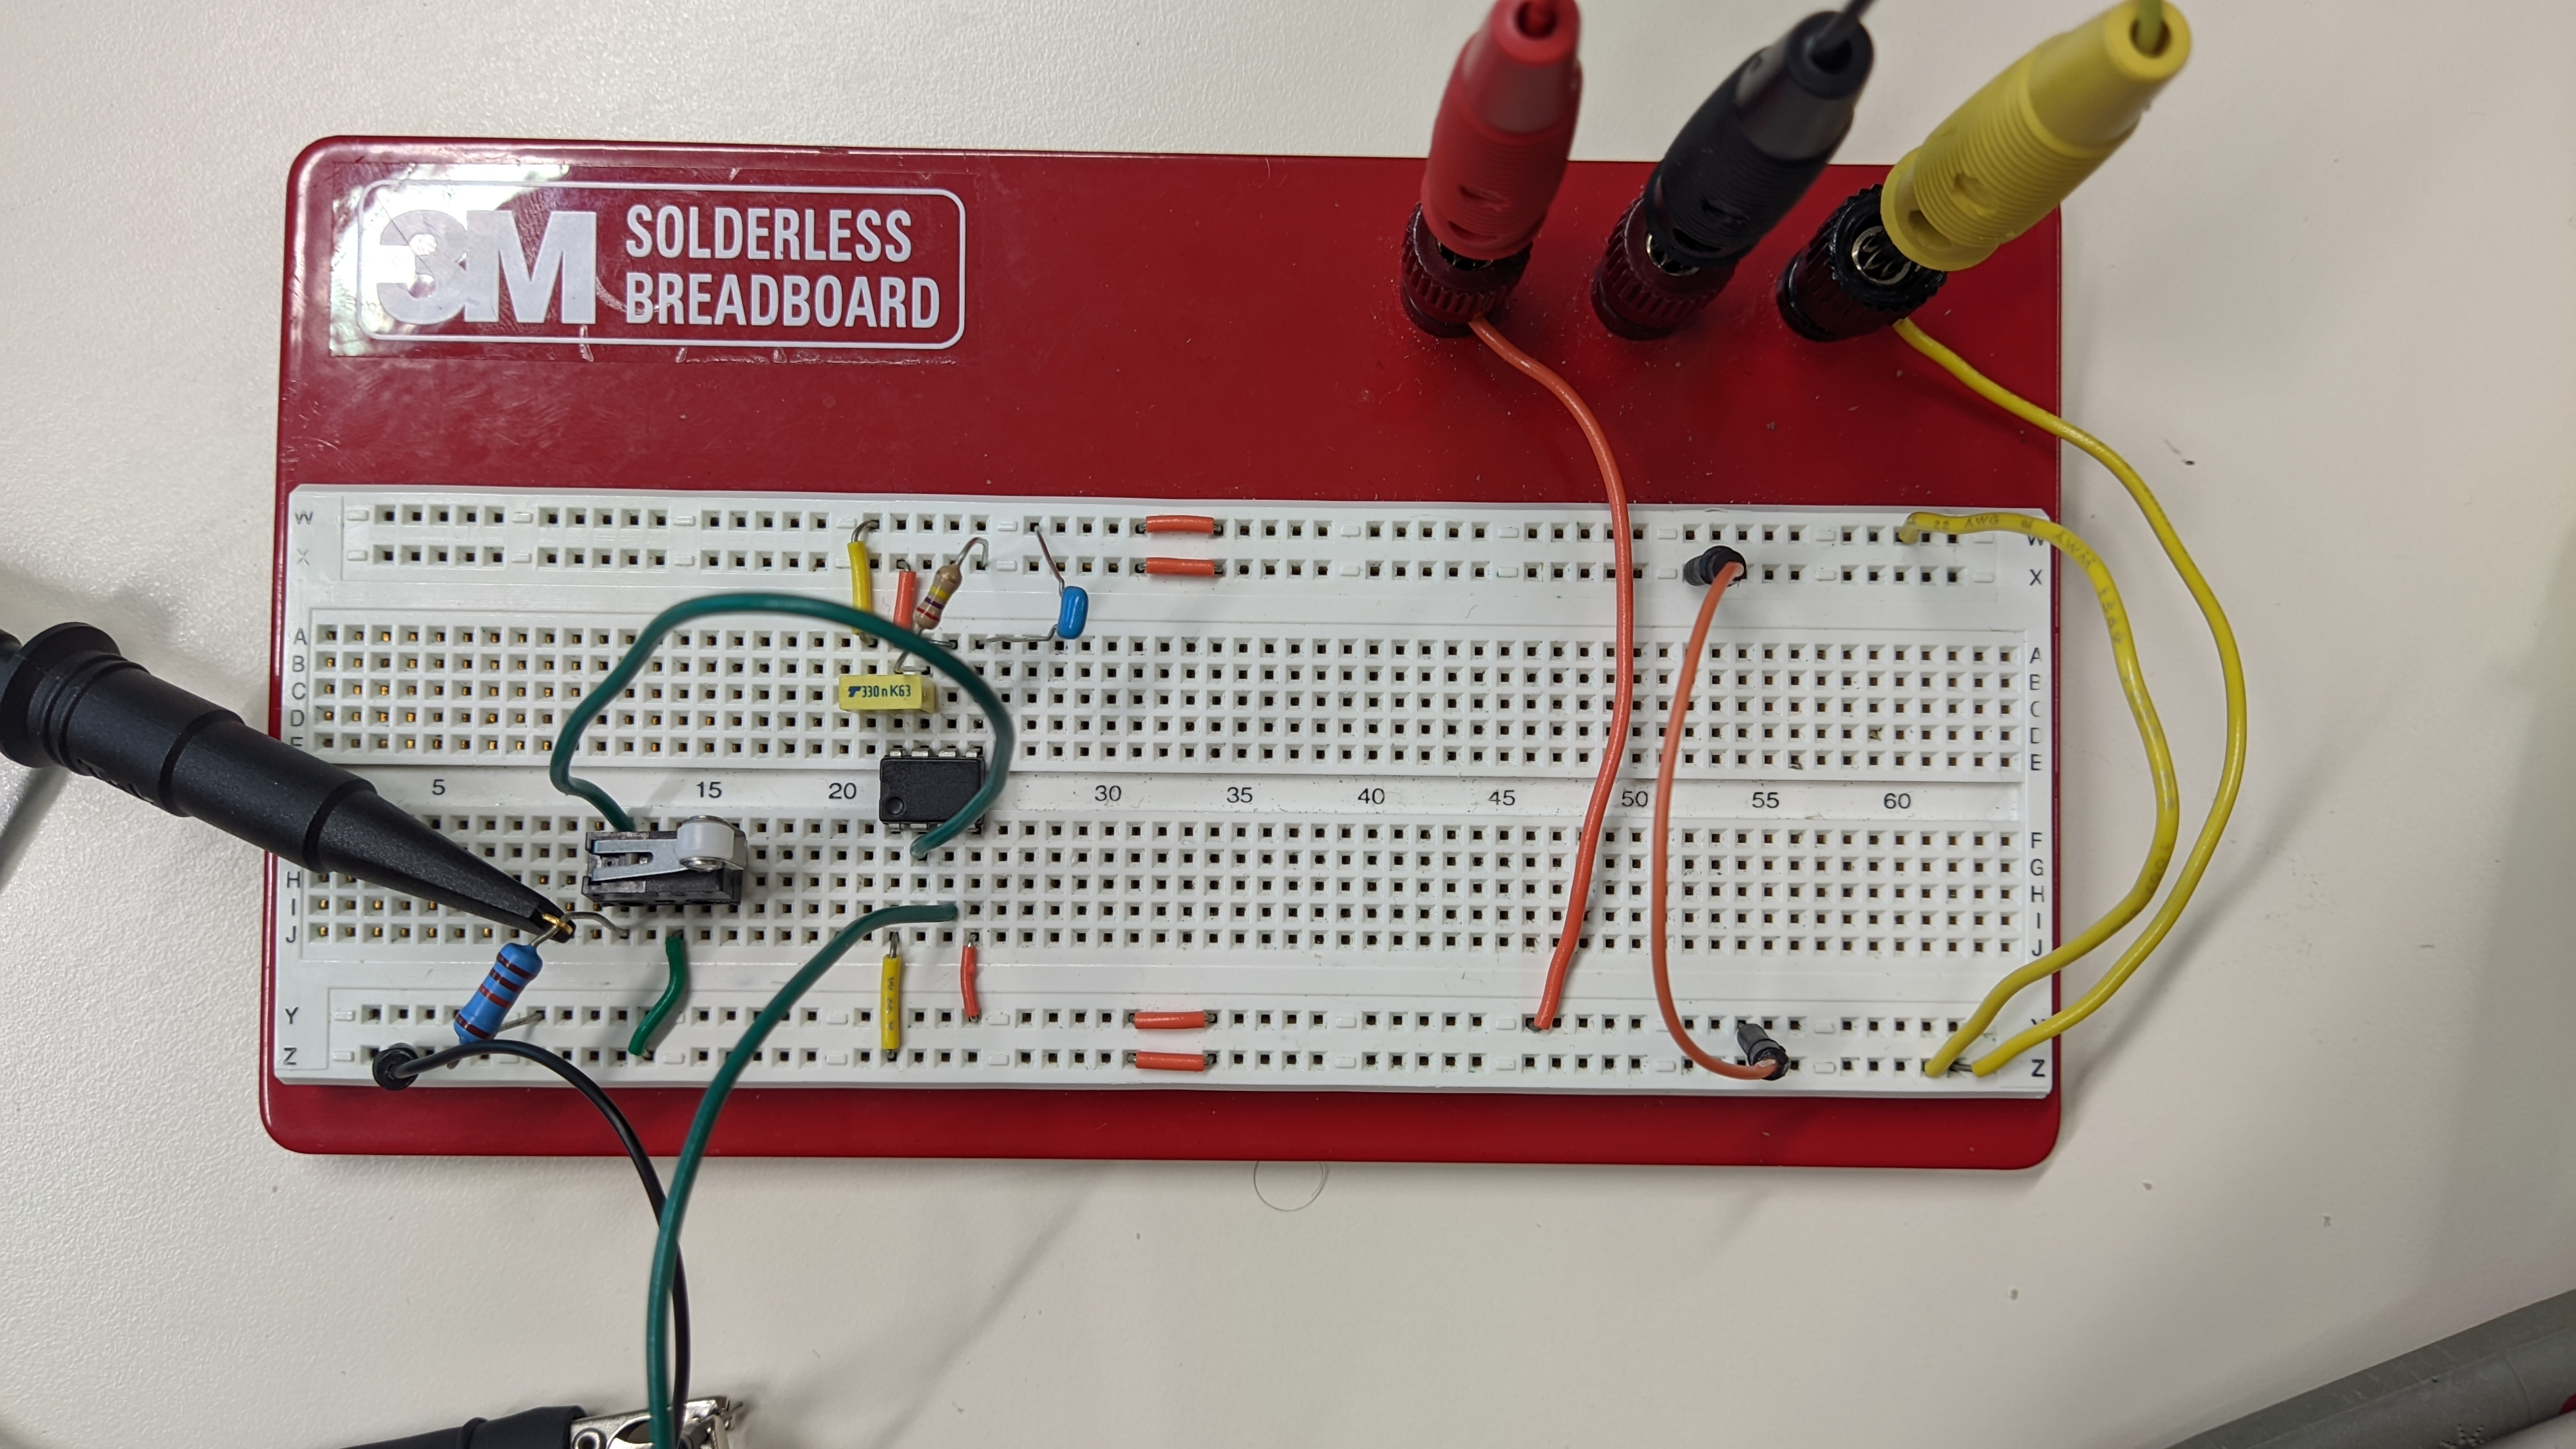
\includegraphics[width=\linewidth]{./ImageFiles/Laboratorio 5/CIR1.jpg}
	\end{minipage}
	\caption{Schema circuitale e foto del circuito realizzato.}
	\label{fig:circuito_1}
\end{figure}

\noindent
In questo circuito il Timer 555 è utilizzato in configurazione monostabile. A differenza del circuito realizzato nella relazione precedente, il segnale di trigger viene generato non più tramite il generatore di forme d'onda ma tramite un pulsante meccanico normalmente aperto. 
Esso ha un terminale connesso alla resistenza $R_2$ di pull-up verso $V_{CC}$, mentre l'altro terminale è connesso a massa. Per cui, quando l'interruttore è aperto sul nodo di \textit{Trigger} viene mantenuta una tensione di $V_{CC}$ grazie alla resistenza $R_2$. Quando l'interruttore viene chiuso invece il morsetto di \textit{Trigger} viene collegato a massa. Tuttavia, la risposta reale di un pulsante meccanico durante l'apertura e la chiusura è influenzata dalla propria risposta meccanica, caratterizzata dal fenomeno del rimbalzo (\textit{switch bouncing}). A causa di questo effetto, si possono notare degli impulsi di apertura-chiusura quando viene premuto o rilasciato il pulsante (\Fig\ref{fig:switch_bouncing}).
\begin{figure}[tbh]
	\centering
	\begin{minipage}{.496\textwidth}
		\includegraphics[width=\linewidth]{./ImageFiles/Laboratorio 5/TEK00003.PNG}
	\end{minipage}
	\begin{minipage}{.496\textwidth}
		\includegraphics[width=\linewidth]{./ImageFiles/Laboratorio 5/TEK00002.PNG}
	\end{minipage}
	\caption{Effetto rimbalzo durante l'apertura e la chiusura di un pulsante meccanico. A sinistra è possibile vedere il segnale ai morsetti del pulsante quando viene premuto per circa \SI{55.2}{\milli\second}. A destra un dettaglio sul segnale alla pressione del pulsante in cui l'effetto del rimbalzo dura circa \SI{478}{\micro\second}.}
	\label{fig:switch_bouncing}
\end{figure}
Questo comportamento anomalo potrebbe presentare un problema quando è inserito, per esempio, in un circuito digitale che conta quante volte è stato premuto il pulsante: il circuito contatore conterà anche le oscillazioni causate dal rimbalzo. Per superare questo problema è possibile sfruttare il LM555 in modalità monostabile che, a seguito di un impulso negativo sul trigger genera un impulso in uscita con durata pari a $T=1.1RC$. Il circuito quindi realizzato può essere utilizzato per ottenere un singolo impulso in uscita a seguito della pressione del pulsante collegato al morsetto di trigger. Nella figura \ref{fig:circuito_1_scope} viene confrontato l'andamento della tensione al morsetto di trigger e la tensione in uscita al timer 555. I valori dei componenti passivi utilizzati per questa misura sono pari a $R_2= R= C=$\todo{completare e confrontare teorico e misurato}. 
\begin{figure}[tbh]
	\centering
	\begin{minipage}{.496\textwidth}
		\includegraphics[width=\linewidth]{./ImageFiles/Laboratorio 5/TEK00005.PNG}
	\end{minipage}
	\begin{minipage}{.496\textwidth}
		\includegraphics[width=\linewidth]{./ImageFiles/Laboratorio 5/TEK00006.PNG}
	\end{minipage}
	\caption{Uscita al LM555 (linea azzurra) in configurazione monostabile e tensione al morsetto di trigger (linea gialla).}
	\label{fig:circuito_1_scope}
\end{figure}



\clearpage
Il secondo circuito realizzato utilizza LM555 in modalità bistabile (\Fig\ref{label}) e permette di generare un impulso rettangolare in uscita al time 555 di durata controllabile dalla pressione di due pulsanti: un pulsante di trigger e uno di reset.
\todo{foto e schema circuito 2}



\begin{figure}[tbh]
	\centering
	\begin{minipage}{.496\textwidth}
		\includegraphics[width=\linewidth]{./ImageFiles/Laboratorio 5/TEK00010.PNG}
	\end{minipage}
	\begin{minipage}{.496\textwidth}
		\includegraphics[width=\linewidth]{./ImageFiles/Laboratorio 5/TEK00011.PNG}
	\end{minipage}
	\caption{}
	\label{fig:circuito_2_scope}
\end{figure}